% !TeX encoding = UTF-8
\documentclass[aspectratio=169]{ctexbeamer}

\mode<presentation>
\usetheme[maxplus,default]{sjtubeamer}

\usepackage{amsmath}
\usepackage{amssymb}
\usepackage{booktabs}
\usepackage{graphicx}
\usepackage{array}
\usepackage{url}

\graphicspath{{../paper_mid/}}

\title{Stabilizing Residual Vector-Quantized Behavior Transformers for Multi-Modal Imitation Learning}
\subtitle{Final Project Presentation}
\author{Sirui Song \and Zhongyu You}
\institute[SJTU]{Shanghai Jiao Tong University}
\date{\today}

\begin{document}

\maketitle

\begin{frame}
  \frametitle{Presentation Roadmap}
  \begin{enumerate}
    \item Problem motivation and background
    \item RVQ-BeT technical approach
    \item Experimental setup: BlockPush and Franka Kitchen
    \item Results and analysis
    \item Key conclusions, limitations, and future work
  \end{enumerate}
\end{frame}

\begin{frame}
  \frametitle{Problem Motivation}
  \framesubtitle{Why multi-modal behavior cloning is difficult}
  \begin{itemize}
    \item In robotic manipulation, the same observation can admit multiple valid actions.
    \begin{itemize}
      \item Different object orders
      \item Different contact points
      \item Different local trajectories
    \end{itemize}
    \item Standard regression policies tend to average across modes.
    \item The average of several valid actions may be invalid.
  \end{itemize}
  \vspace{0.5em}
  \begin{block}{Core question}
    Can we represent multi-modal continuous actions with a better discrete latent action space?
  \end{block}
\end{frame}

\begin{frame}
  \frametitle{Background: Behavior Transformer}
  \framesubtitle{Discrete action bin + continuous offset}
  \begin{columns}[T]
    \begin{column}{0.52\textwidth}
      \begin{itemize}
        \item BeT clusters continuous actions using $k$-means.
        \item The policy predicts:
        \begin{itemize}
          \item a discrete action bin;
          \item a residual continuous offset.
        \end{itemize}
        \item This converts multi-modal action prediction into classification plus local regression.
      \end{itemize}
    \end{column}
    \begin{column}{0.42\textwidth}
      \begin{block}{BeT action prediction}
      \begin{equation*}
        \hat{a}_t = A_{c_t} + \Delta a_t
      \end{equation*}
      \end{block}
      \begin{alertblock}{Limitation}
        The action tokenizer is fixed by $k$-means.
      \end{alertblock}
    \end{column}
  \end{columns}
\end{frame}

\begin{frame}
  \frametitle{Project Goal}
  \framesubtitle{A controlled adaptation of VQ-style latent actions}
  \begin{block}{Research question}
    Can a learned residual vector-quantized tokenizer replace BeT's fixed $k$-means tokenizer while keeping the transformer backbone unchanged?
  \end{block}
  \vspace{0.6em}
  \begin{itemize}
    \item Keep the GPT-like transformer policy backbone fixed.
    \item Modify only:
    \begin{itemize}
      \item action tokenizer;
      \item RVQ code prediction heads;
      \item offset-conditioning pathway.
    \end{itemize}
    \item This isolates the effect of the latent action interface.
  \end{itemize}
\end{frame}

\begin{frame}
  \frametitle{RVQ Action Tokenizer}
  \framesubtitle{Hierarchical discrete latent actions}
  \begin{columns}[T]
    \begin{column}{0.52\textwidth}
      \begin{itemize}
        \item Encode action: $x_t=f_{\mathrm{enc}}(a_t)$.
        \item Quantize with one or two codebooks.
        \item Decode selected code embeddings into an action center.
        \item Predict final action with a residual offset.
      \end{itemize}
      \begin{equation*}
        \hat{a}_t = f_{\mathrm{dec}}\left(\sum_i e_{z_t^{(i)}}^{(i)}\right) + \hat{o}_t
      \end{equation*}
    \end{column}
    \begin{column}{0.42\textwidth}
      \begin{block}{$N_q=2$ residual quantization}
      \begin{align*}
        z_t^{(1)} &= \arg\min_k \|x_t-e_k^{(1)}\|_2^2 \\
        r_t^{(1)} &= x_t-e_{z_t^{(1)}}^{(1)} \\
        z_t^{(2)} &= \arg\min_k \|r_t^{(1)}-e_k^{(2)}\|_2^2
      \end{align*}
      \end{block}
    \end{column}
  \end{columns}
\end{frame}

\begin{frame}
  \frametitle{Midterm Diagnosis: Code Collapse}
  \framesubtitle{The first RVQ versions failed for a representation reason}
  \begin{itemize}
    \item Early RVQ variants achieved only around $0.16/0.17$ reward on BlockPush.
    \item Diagnostics showed that most actions were assigned to one code.
    \item The discrete latent stopped representing action modes.
    \item The policy became approximately:
    \begin{equation*}
      \text{constant action center} + \text{large offset regressor}
    \end{equation*}
  \end{itemize}
  \begin{alertblock}{Key lesson}
    Before comparing RVQ with $k$-means, the learned codebook must be verified to avoid collapse.
  \end{alertblock}
\end{frame}

\begin{frame}
  \frametitle{Stabilization Strategy}
  \framesubtitle{Making RVQ usable inside BeT}
  \begin{columns}[T]
    \begin{column}{0.48\textwidth}
      \begin{block}{Residual $k$-means initialization}
        \begin{itemize}
          \item $N_q=1$: initialize on encoder latents.
          \item $N_q=2$: initialize second codebook on residuals.
        \end{itemize}
      \end{block}
      \begin{block}{Dead-code restart}
        Reinitialize unused codes with high-error samples.
      \end{block}
    \end{column}
    \begin{column}{0.48\textwidth}
      \begin{block}{Diagnostics}
        \begin{itemize}
          \item Active code count
          \item Perplexity
          \item Maximum usage ratio
          \item Reconstruction error
        \end{itemize}
      \end{block}
      \begin{block}{Goal}
        Ensure discrete codes carry meaningful action structure.
      \end{block}
    \end{column}
  \end{columns}
\end{frame}

\begin{frame}
  \frametitle{Offset-Conditioning Variants}
  \framesubtitle{How should discrete codes interact with continuous offsets?}
  \small
  \begin{table}
  \centering
  \resizebox{0.95\textwidth}{!}{%
  \begin{tabular}{lll}
  \toprule
  Variant & RVQ depth & Offset conditioning \\
  \midrule
  Code-independent & $N_q=1,2$ & Hidden state only \\
  Code-dependent & $N_q=1$ & Branch selected by predicted code \\
  Primary-dependent & $N_q=2$ & Branch selected by first code \\
  Code-embedding-conditioned & $N_q=2$ & Hidden state plus selected code embeddings \\
  \bottomrule
  \end{tabular}}
  \end{table}
  \vspace{0.5em}
  \begin{block}{Hypothesis}
    The offset should refine the selected latent action mode, not independently reconstruct the whole action.
  \end{block}
\end{frame}

\begin{frame}
  \frametitle{Experimental Setup}
  \framesubtitle{Two complementary environments}
  \begin{columns}[T]
    \begin{column}{0.48\textwidth}
      \begin{block}{BlockPush}
        \begin{itemize}
          \item Low-dimensional multi-modal pushing.
          \item Main midterm environment.
          \item $K=16$.
          \item 120 evaluation episodes.
          \item Used to diagnose and stabilize RVQ.
        \end{itemize}
      \end{block}
    \end{column}
    \begin{column}{0.48\textwidth}
      \begin{block}{Franka Kitchen}
        \begin{itemize}
          \item State-based \texttt{kitchen-all-v0}.
          \item Observation dimension: 60.
          \item Action dimension: 9.
          \item $K=64$.
          \item 100 evaluation episodes.
        \end{itemize}
      \end{block}
    \end{column}
  \end{columns}
\end{frame}

\begin{frame}
  \frametitle{BlockPush Results}
  \framesubtitle{RVQ recovers from collapse but does not beat $k$-means}
  \small
  \begin{table}
  \centering
  \resizebox{0.95\textwidth}{!}{%
  \begin{tabular}{lcc}
  \toprule
  Configuration & Avg. Reward & Success$_{\ge 0.99}$ \\
  \midrule
  BeT + $k$-means ($K=16$) & 0.8647 & 92/120 \\
  RVQ $N_q=1$ code-independent & 0.7676 & 73/120 \\
  RVQ $N_q=1$ code-dependent & 0.8177 & 80/120 \\
  RVQ $N_q=2$ primary-dependent & 0.7592 & 73/120 \\
  RVQ $N_q=2$ code-embedding-conditioned & 0.8142 & 83/120 \\
  \bottomrule
  \end{tabular}}
  \end{table}
  \begin{itemize}
    \item Collapse-stage RVQ: around $0.16/0.17$ reward.
    \item Stabilized RVQ: reaches $0.76$--$0.81$ range.
    \item Best RVQ variants use code-conditioned offsets.
  \end{itemize}
\end{frame}

\begin{frame}
  \frametitle{BlockPush Diagnostics and Visualization}
  \framesubtitle{Collapse was mitigated, but rollout quality still differs}
  \begin{columns}[T]
    \begin{column}{0.48\textwidth}
      \begin{itemize}
        \item Stabilized tokenizers use all 16 codes.
        \item Example $N_q=2$ diagnostics:
        \begin{itemize}
          \item Primary code PPL: 13.98--14.78
          \item Secondary code PPL: 11.18--12.08
          \item Max usage ratio below 0.19
        \end{itemize}
        \item Remaining gap likely involves code prediction and offset use.
      \end{itemize}
    \end{column}
    \begin{column}{0.48\textwidth}
      \centering
      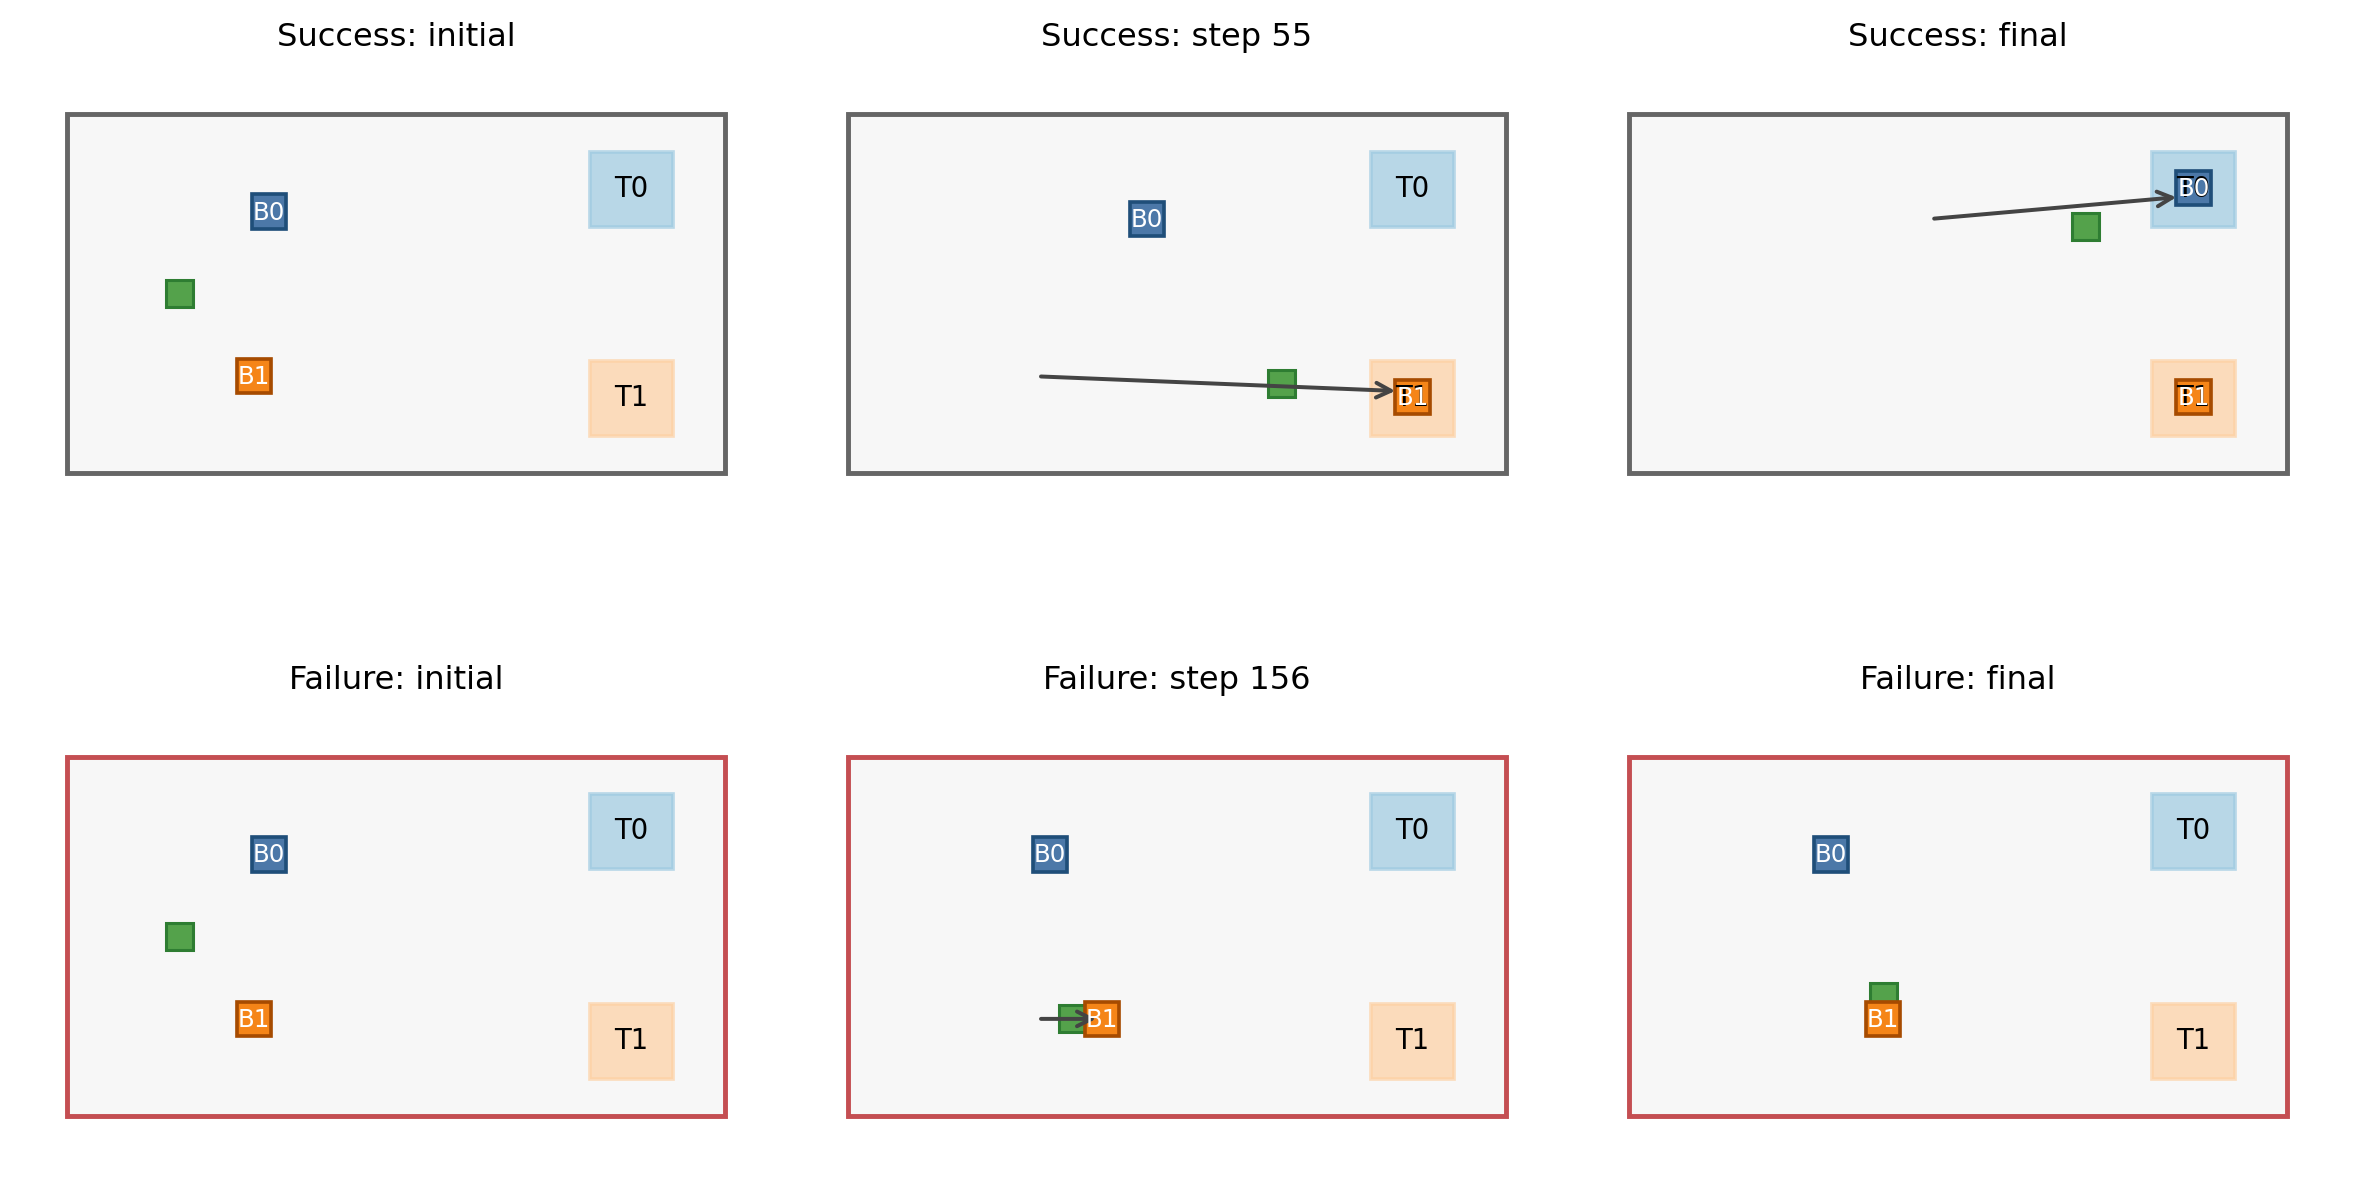
\includegraphics[width=\textwidth]{blockpush_success_failure_diagram.png}
      \vspace{0.2em}
      {\scriptsize Successful rollouts establish contact early; failed rollouts often delay interaction.}
    \end{column}
  \end{columns}
\end{frame}

\begin{frame}
  \frametitle{Franka Kitchen Results}
  \framesubtitle{RVQ becomes competitive in a richer environment}
  \small
  \begin{table}
  \centering
  \resizebox{0.95\textwidth}{!}{%
  \begin{tabular}{lcc}
  \toprule
  Configuration & Avg. Reward & Std. \\
  \midrule
  BeT + $k$-means ($K=64$) & 2.92 & 1.1548 \\
  RVQ $N_q=1$ code-independent & 2.00 & 1.4353 \\
  RVQ $N_q=1$ code-dependent & 3.00 & 1.1314 \\
  RVQ $N_q=2$ code-independent & 1.59 & 1.1755 \\
  RVQ $N_q=2$ primary-dependent & 1.78 & 1.2213 \\
  RVQ $N_q=2$ code-embedding-conditioned & 3.05 & 0.9631 \\
  \bottomrule
  \end{tabular}}
  \end{table}
  \begin{itemize}
    \item Best result: $N_q=2$ code-embedding-conditioned RVQ.
    \item $N_q=1$ code-dependent RVQ is also comparable to baseline.
    \item Code-independent variants perform substantially worse.
  \end{itemize}
\end{frame}

\begin{frame}
  \frametitle{Cross-Environment Analysis}
  \framesubtitle{What changed from BlockPush to Kitchen?}
  \begin{columns}[T]
    \begin{column}{0.48\textwidth}
      \begin{block}{BlockPush}
        \begin{itemize}
          \item Low-dimensional actions.
          \item $K=16$ $k$-means may already cover action modes well.
          \item RVQ adds prediction complexity without clear gain.
        \end{itemize}
      \end{block}
    \end{column}
    \begin{column}{0.48\textwidth}
      \begin{block}{Kitchen}
        \begin{itemize}
          \item Higher-dimensional actions.
          \item Multiple subtasks and richer action structure.
          \item Hierarchical RVQ can become useful when offsets use both codes.
        \end{itemize}
      \end{block}
    \end{column}
  \end{columns}
  \vspace{0.5em}
  \begin{alertblock}{Caution}
    The Kitchen improvement is small relative to rollout variance; it indicates potential, not conclusive superiority.
  \end{alertblock}
\end{frame}

\begin{frame}
  \frametitle{Key Findings}
  \begin{enumerate}
    \item \textbf{Code collapse was the main initial failure mode.}
    \begin{itemize}
      \item Stabilization is necessary before meaningful comparison.
    \end{itemize}
    \item \textbf{Offset conditioning is crucial.}
    \begin{itemize}
      \item Code-conditioned offsets consistently outperform code-independent variants.
    \end{itemize}
    \item \textbf{Environment complexity matters.}
    \begin{itemize}
      \item RVQ does not clearly beat $k$-means on BlockPush.
      \item RVQ becomes competitive and slightly better on Kitchen.
    \end{itemize}
  \end{enumerate}
\end{frame}

\begin{frame}
  \frametitle{Limitations and Future Directions}
  \begin{columns}[T]
    \begin{column}{0.48\textwidth}
      \begin{alertblock}{Limitations}
        \begin{itemize}
          \item Mostly single-seed results.
          \item Kitchen lacks tokenizer diagnostics.
          \item No Kitchen code prediction accuracy yet.
          \item Reward alone does not reveal subtask behavior.
        \end{itemize}
      \end{alertblock}
    \end{column}
    \begin{column}{0.48\textwidth}
      \begin{block}{Future work}
        \begin{itemize}
          \item Multi-seed evaluation.
          \item Kitchen code usage and perplexity diagnostics.
          \item Subtask-level completion analysis.
          \item Better $N_q=2$ training strategies.
        \end{itemize}
      \end{block}
    \end{column}
  \end{columns}
\end{frame}

\begin{frame}
  \frametitle{Conclusion}
  \begin{itemize}
    \item RVQ tokenization can be integrated into BeT, but requires stabilization.
    \item On BlockPush, RVQ approaches but does not surpass $k$-means.
    \item On Franka Kitchen, code-conditioned RVQ achieves comparable or slightly better reward.
    \item Learned hierarchical tokenization may become more useful in higher-dimensional, multi-stage manipulation tasks.
  \end{itemize}
  \vspace{0.8em}
  \begin{block}{Takeaway}
    The key challenge is not only learning discrete action codes, but aligning them with the continuous offset pathway used for action reconstruction.
  \end{block}
\end{frame}

\begin{frame}
  \frametitle{Project Repository}
  \begin{center}
    \Large \url{https://github.com/gradient-1024/RVQ_bet}
  \end{center}
  \vspace{1em}
  \begin{center}
    \Huge Thank you!
  \end{center}
\end{frame}

\end{document}
